\documentclass[a4paper,12pt]{article}
\usepackage[utf8]{inputenc}
\usepackage[T1]{fontenc}
\usepackage{lmodern}
\usepackage{amsmath}
\usepackage{geometry}
\usepackage{booktabs}
\usepackage{graphicx}
\usepackage{enumitem}
\usepackage{xcolor}
\geometry{margin=2.5cm}
\setlength{\parindent}{0pt}
\setlength{\parskip}{0.6em}
\usepackage{amsmath}
\usepackage{booktabs}
\usepackage{pgfplots}
\pgfplotsset{compat=1.18}
\usepackage{float}

\title{IoT - Challenge 4 Homework - Part 3}
\author{Raul Agolli - Team Leader \\\\ Gabriele Lorenzo Singe}
\date{May 2026}

\begin{document}

\maketitle
\section{Exercise 3 -- RFID}

\subsection{Problem Statement}

An RFID system based on Dynamic Frame ALOHA is composed of:

\[
N=4
\]

tags. The objective is to compute the overall collision resolution efficiency:

\[
\eta = \frac{N}{L(N)}
\]

for different values of the initial frame size:

\[
r_1 = 1,2,3,4,5,6
\]

In RFID systems, when multiple tags answer at the same time, collisions occur and an arbitration mechanism is required to identify all tags. In Frame ALOHA, each frame is composed of \(r\) slots and each tag randomly chooses one slot in which to transmit. If a tag is alone in a slot, it is successfully identified. If two or more tags choose the same slot, a collision occurs and those tags remain in the backlog.

The exercise assumes that after the first frame, the frame size is correctly set equal to the current backlog size.

The following values are given:

\[
L_2 = 4
\]

\[
L_3 = \frac{51}{8}
\]

Moreover:

\[
L_0 = 0
\]

\[
L_1 = 1
\]

\subsection{Recursive Computation of the Arbitration Period}

Let \(L_N(r_1)\) be the expected length of the arbitration period when the initial number of tags is \(N=4\) and the initial frame size is \(r_1\).

After the first frame, some tags may be successfully identified, while the remaining tags form the backlog.

Let \(B\) be the number of tags still unresolved after the first frame. Then:

\[
L_4(r_1) = r_1 + \sum_{b=0}^{4} P(B=b) L_b
\]

where \(P(B=b)\) is the probability that \(b\) tags remain in the backlog after the first frame.

The efficiency is then computed as:

\[
\eta(r_1)=\frac{4}{L_4(r_1)}
\]

\subsection{Computation of \(L_4\)}

Since after the first frame the frame size is correctly set equal to the current backlog size, we first need the value of \(L_4\), corresponding to the case where the backlog is \(4\) and the frame size is also \(4\).

For \(N=4\) tags and \(r=4\) slots, the probabilities of the residual backlog after one frame are:

\[
P(B=0)=\frac{3}{32}
\]

\[
P(B=2)=\frac{9}{16}
\]

\[
P(B=3)=\frac{3}{16}
\]

\[
P(B=4)=\frac{5}{32}
\]

Therefore:

\[
L_4 = 4 + P(B=0)L_0 + P(B=2)L_2 + P(B=3)L_3 + P(B=4)L_4
\]

Substituting the known values:

\[
L_4 =
4
+
\frac{3}{32} \cdot 0
+
\frac{9}{16} \cdot 4
+
\frac{3}{16} \cdot \frac{51}{8}
+
\frac{5}{32} L_4
\]

\[
L_4 =
4
+
\frac{9}{4}
+
\frac{153}{128}
+
\frac{5}{32}L_4
\]

Moving the recursive term to the left-hand side:

\[
L_4 - \frac{5}{32}L_4 =
4
+
\frac{9}{4}
+
\frac{153}{128}
\]

\[
\frac{27}{32}L_4 =
\frac{953}{128}
\]

Thus:

\[
L_4 =
\frac{953}{108}
\]

\[
L_4 \approx 8.8241
\]

\subsection{Efficiency for Different Initial Frame Sizes}

For each initial frame size \(r_1\), we compute:

\[
L_4(r_1) = r_1 + \sum_{b=0}^{4} P(B=b)L_b
\]

and then:

\[
\eta(r_1)=\frac{4}{L_4(r_1)}
\]

The resulting values are reported in Table~\ref{tab:rfid_efficiency}.

\begin{table}[H]
\centering
\begin{tabular}{c c c}
\toprule
Initial frame size \(r_1\) & \(L_4(r_1)\) & Efficiency \(\eta\) \\
\midrule
1 & \(9.8241\) & \(0.4072\) \\
2 & \(9.5995\) & \(0.4167\) \\
3 & \(8.9544\) & \(0.4467\) \\
4 & \(8.8241\) & \(0.4533\) \\
5 & \(9.0377\) & \(0.4426\) \\
6 & \(9.4661\) & \(0.4226\) \\
\bottomrule
\end{tabular}
\caption{Collision resolution efficiency for different initial frame sizes.}
\label{tab:rfid_efficiency}
\end{table}

\subsection{Efficiency Plot}

Figure~\ref{fig:rfid_efficiency} shows the efficiency \(\eta\) as a function of the initial frame size \(r_1\).

\begin{figure}[H]
\centering
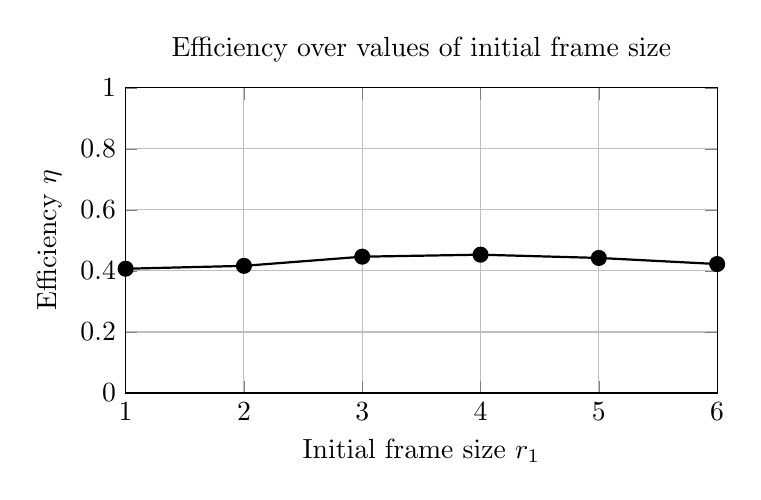
\begin{tikzpicture}
\begin{axis}[
    width=0.75\textwidth,
    height=0.45\textwidth,
    xlabel={Initial frame size \(r_1\)},
    ylabel={Efficiency \(\eta\)},
    title={Efficiency over values of initial frame size},
    xmin=1, xmax=6,
    ymin=0, ymax=1,
    xtick={1,2,3,4,5,6},
    ytick={0,0.2,0.4,0.6,0.8,1.0},
    grid=both,
    mark size=2.5pt
]
\addplot[
    mark=*,
    thick
]
coordinates {
    (1,0.4072)
    (2,0.4167)
    (3,0.4467)
    (4,0.4533)
    (5,0.4426)
    (6,0.4226)
};
\end{axis}
\end{tikzpicture}
\caption{Efficiency \(\eta\) over the initial frame size \(r_1\).}
\label{fig:rfid_efficiency}
\end{figure}

\subsection{Maximum Efficiency}

From Table~\ref{tab:rfid_efficiency}, the maximum value of the efficiency is obtained for:

\[
r_1 = 4
\]

The corresponding efficiency is:

\[
\eta_{\max} = 0.4533
\]

Therefore:

\[
\boxed{r_1^{\star}=4}
\]

\[
\boxed{\eta_{\max}=0.4533}
\]

\subsection{Comment}

The maximum efficiency is obtained when the initial frame size is equal to the number of tags:

\[
r_1 = N = 4
\]

This result is consistent with the behavior of Frame ALOHA. If the frame size is too small, many tags choose the same slots, increasing the number of collisions. If the frame size is too large, many slots remain empty, wasting time. Therefore, the best trade-off is achieved when the frame size is close to the number of contending tags.

In this case, since \(N=4\), the best initial choice is:

\[
\boxed{r_1 = 4}
\]

\subsection{Final Results}

The final efficiency values are:

\[
\boxed{
\begin{aligned}
\eta(1) &= 0.4072 \\
\eta(2) &= 0.4167 \\
\eta(3) &= 0.4467 \\
\eta(4) &= 0.4533 \\
\eta(5) &= 0.4426 \\
\eta(6) &= 0.4226
\end{aligned}
}
\]

The maximum efficiency is:

\[
\boxed{\eta_{\max}=0.4533}
\]

and it is obtained for:

\[
\boxed{r_1=4}
\]

\end{document}